\section*{Samsung macht die Schule smart?}
\label{smartschool}
\NewsAuthor{Martin Mayr}

\textbf{Martin Mayr macht sich in seinem \href{http://martinslangweiligesblog.wordpress.com/2013/04/01/the-future-of-education-powered-by-samsung/}{\textit{Blogposting [1]}} vom April 2013 ein wenig lustig über die Samsung Smartschool Initiative im Bildungsbereich. Originaltitel: 'The future of education, powered by Samsung". Martin lebt in Wien und beschäftigt sich mit Ernährungssouveränität, Urban Gardening sowie Montessori-Pädagogik. Er betreibt einen Blog und ist manchmal zu Gast im \href{http://biertaucher.at}{\textit{Biertaucher-Podcast [2]}}.}

\begin{center}
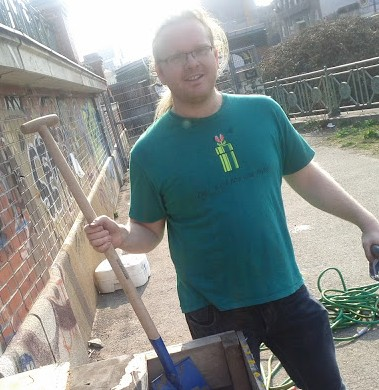
\includegraphics[width=\linewidth]{smartschool/martinderm2.jpg} \\
\footnotesize{Martin Mayr. Bildrechte: \href{http://spielend-programmieren.at}{Horst JENS}[3] \href{http://creativecommons.org/licenses/by-sa/3.0/}{cc-by-sa}}
\end{center}

(Beginn des Original-Textes)\\

%\paragraph{}
Eine Antwort auf einen \href{http://futurezone.at/digital-life/ideenwettbewerb-einreichen-und-abstimmen/24.593.816}{\textit{Futurezone Bericht über Smartschools [4]}}.

%\footnote{l{http://futurezone.at/digital-life/ideenwettbewerb-einreichen-und-abstimmen/24.593.816}}. 

%\paragraph{}
\emph{Wie soll das Klassenzimmer der Zukunft aussehen, wie soll es funktionieren und wie stellen sich Schüler den Unterricht vor?} - Das frage ich mich auch schon lange. Das Spektrum der Lösungen soll nun von \href{http://futurezone.at/digitallife/14934-eboards-und-tablets-fuer-die-besten-ideen.php}{\textit{zwei relativ neuen Akteuren [5]}}  gefunden werden: \href{http://futurezone.at/}{\textit{Futurezone}} und Samsung starten den Ideenwettbewerb \emph{Samsung Smart School}, der vom Bundesministerium für Unterricht, Kunst und Kultur unterstützt wird.

%\paragraph{}
Der Technologiekonzern lanciert so wie es aussieht eine internationale Kampagne ( \href{http://www.samsung.com/global/business/business-images/resource/RR-BC/2012/10/SamsungSmartSchoolLeaflet-0.pdf}{\textit{siehe Leaflet [6]}}) 
%\footnote{\url{http://www.samsung.com/global/business/business-images/resource/RR-BC/2012/10/SamsungSmartSchoolLeaflet-0.pdf}}
um seine Produkte in die Klassenzimmer der Welt zu bekommen, und in Österreich springen Medien wie Ministerien, im Angesicht der allgemeinen Ratlosigkeit bei der Bewältigung der vielfältigen Probleme im Bildungssystem, mit größter Freude auf.

%\paragraph{}
Wie soll die Schule der Zukunft nun also aussehen?
\begin{quote}\glqq 
Österreichweit sind alle Volksschulen und alle Mittel- und Oberstufen eingeladen, sich Gedanken über die Schule der Zukunft, über den Unterricht der Zukunft, über mobile Lösungen und den interaktiven Unterricht und selbstbestimmtes Lernen außerhalb des Unterrichts zu machen.\grqq
\end{quote}

Selbstbestimmtes Lernen soll aber außerhalb des Unterrichts stattfinden? Genau dort hat selbstbestimmtes Lernen schon immer stattgefunden und wird durch neue Technologieen nicht zwangsläufig verbessert.

%\paragraph{}
Als Erzfeind wurde vollkommen richtig der Frontalunterricht identifiziert, ob neue Lernkonzepte ihren Weg in den Schulalltag finden werden \href{http://futurezone.at/digitallife/14938-gesucht-die-smarte-schule-von-morgen.php}{\textit{bleibt aber offen [4]}}
%\footnote{\url{http://futurezone.at/digitallife/14938-gesucht-die-smarte-schule-von-morgen.php}\label{fuzomorgen}}.
Samsung schreitet nun gottlob als weiser Ritter heran, um uns von der kinderverblödenden Kreidetafel zu erlösen. Dies erfolgt umsatzsteigernd durch Tablets, Pads, Slates oder PCs, in Kooperation mit Bundesministerium für Unterricht, Kunst und Kultur sowie futurezone.at.

%\paragraph{}
Eine kleine Auswahl was uns in diesem Sinne erwartet: (Quellen: \href{http://futurezone.at/digitallife/14938-gesucht-die-smarte-schule-von-morgen.php}{\textit{Futurezone [4]}},
\href{http://futurezone.at/digitallife/14960-tablet-und-pc-klassen-als-vorzeigeprojekte.php}{\textit{Futurezone [7]}})


\begin{itemize}
  \item "…es [ist] nun möglich, dem Lehrer … auf privatem Wege Fragen zu stellen"
  \item "…eine integrierte Lernplattform, mit der Lehrer und Schüler in einer interaktiven Umgebung arbeiten können."
  \item "das Wort … von einem Native Speaker vorgelesen …"
\end{itemize}

%\paragraph{}
Bleibt die Frage: Welche heute im Klassenzimmer abwesende Technologie hindert unsere Gesellschaft daran diese Erfahrungen den Schülern zu bieten?

%\paragraph{}
Aber welche Umgebung soll nun laut Samsung den Schulalltag zum Besseren wenden?
Die \href{http://futurezone.at/digitallife/14938-gesucht-die-smarte-schule-von-morgen.php}{Futurezone  Bildergalerie}[4] gibt Aufschluss darüber: Das Ersetzen von grünen Tafeln, Kreiden und Schulbüchern durch \textbf{Smartboards} und \textbf{Tablets} soll die Lernerfolge unserer SchülerInnen verbessern (oder doch ein neues Geschäftsfeld erschliessen?).

%\paragraph{}
Als 'integrierte Lernplattform' kommt mir das, mit einigem guten Willen, bekannt vor. Im \href{http://www.montessori-kindergarten.at/}{\textit{Montessori Kinderhaus [8]}} wird so gelernt, jedes Kind mit einem Material, welches bis ins kleinste Detail wohlüberlegt konstruiert vom absorbierenden Geist verinnerlicht wird. Die perfekte vorbereitete Umgebung. Wenn nicht der Tablet die Repräsentanz aller Lehrmaterialien wäre, als denkbar ungeeignetste Möglichkeit Inhalte an Kindergartenkinder zu Vermitteln.

%\paragraph{}
Leider ist so eine Umgebung für Kinder im Volksschulalter alles andere als geeignet. Montessori hat aus gutem Grund für jede Altersgruppe ein neues, aber auf ihren Erkenntnissen beruhendes Konzept erarbeitet. Und dass jedes Kind alleine vorm Lehrmaterial sitzt gehört für dieses Alter jedenfalls nicht dazu. Ganz im Gegenteil, die Kinder erarbeiten ihr wissen selbstständig, in Kleinstgruppen und nutzen dafür vielfältige Materialien und Quellen.

%\paragraph{}
Samsungs Vision von der Schule der Zukunft aber bleibt eine Erweiterung des Bildungssystems wie wir es in den letzten Jahrzehnten beobachtet haben. Die Schule der Zukunft erfordert nämlich keine neuen Technologien sondern einen grundlegend neuen Zugang zu der Art und Weise wie Bildung vermittelt wird. Und warum dieser gerade von einem Technologiekonzern in die Welt gebracht werden soll muss zumindest ausgiebig hinterfragt werden.

Eine \href{https://vimeo.com/40791188}{\textit{andere Antwort [9]}} 
%\footnote{\url{https://vimeo.com/40791188}}
liefert Stephen Hughes, der als Kinder-Neuropsychologe vielleicht ein klein wenig qualifizierter ist, sich zu diesem Thema zu äußern.
\subsection*{Fachbegriffe:}
\href{https://de.wikipedia.org/wiki/Smartboard#Digitale_Whiteboards}{\textbf{Smartboards} oder \textbf{digitale Whiteboards}}: Elektronische Schultafel, meist eine Kombination aus vertikalem Bildschirm bzw. Projektorfläche für Beamer und geeigneten Eingabemedium in Form eines Stiftes sowie spezieller Software. Statt den Computer per Maus oder Touchpad zu bedienen kann an der vertikalen 'Tafel' am Computer wie mit Kreide 'gemalt' werden.

\href{https://de.wikipedia.org/wiki/Tablet-Computer}{\textbf{Tablet}}: Jeder flache, nur aus beführungsempfindlichem (Touch)-Bildschirm bestehender Computer, z.B. \href{https://de.wikipedia.org/wiki/Apple_iPad}{Apple's IPad}


\subsection*{Download, Feedback:}
\footnotesize{
Download: Ordner \texttt{smartschool} \Mundus\ \href{http://spielend-programmieren.at/risjournal/001}{spielend-programmieren.at/risjournal/001}\\
Startseite:\\
\href{http://spielend-programmieren.at/de:ris:001:start}{spielend-programmieren.at/de:ris:001:start}\\ 
\Letter\: martindermayr@gmail.com\\}
\normalsize 

\subsection*{Lizenz, Quellen:}
\begin{wrapfigure}{l}{2.0cm}

\includegraphics[width=2cm]{smartschool/ccbysa88x31.png}
\end{wrapfigure}
Dieses Material steht unter der Creative-Commons-Lizenz Namensnennung - Weitergabe unter gleichen Bedingungen 4.0 International. Um eine Kopie dieser Lizenz zu sehen, besuchen Sie \url{http://creativecommons.org/licenses/by-sa/4.0/deed.de}.

\textbf{Quellen:} \\
{[}1{]} \url{http://goo.gl/1zMxod} \\
%{http://martinslangweiligesblog.wordpress.com/2013/04/01/the-future-of-education-powered-by-samsung/}
{[}2{]} \url{http://biertaucher.at} \\
{[}3{]} \href{http://spielend-programmieren.at}{spielend-programmieren.at} \\
{[}4{]} \url{http://goo.gl/Q42rbW} \\
%{http://futurezone.at/digitallife/14938-gesucht-die-smarte-schule-von-morgen.php}
{[}5{]} \url{http://goo.gl/WrHB4i} \\
%{http://futurezone.at/digitallife/14934-eboards-und-tablets-fuer-die-besten-ideen.php}
{[}6{]} \url{http://goo.gl/Ev9j0u} \\
%{http://www.samsung.com/global/business/business-images/resource/RR-BC/2012/10/SamsungSmartSchoolLeaflet-0.pdf}
{[}7{]} \url{http://goo.gl/c6v2BA} \\
%http://futurezone.at/digitallife/14960-tablet-und-pc-klassen-als-vorzeigeprojekte.php}
{[}8{]} \href{http://www.montessori-kindergarten.at/}{montessorie-kindergarten.at} \\
{[}9{]} \url{https://vimeo.com/40791188} 



